\documentclass{ecnreport}

\stud{OD Robotique 2020-2021}
\topic{ROS 2 exam}

\begin{document}

\inserttitle{ROS 2 exam}

\insertsubtitle{2h, documents / internet allowed (closed chats please)}


\section{Description}

In this exam you will have to write a C++ node and run it two times through a launch file.\\
As usual with ROS exams at Centrale Nantes, some StarWars robots are featured and should follow each other in this order:
\begin{center}
 d0 $\rightarrow$ bb8 $\rightarrow$ r2d2
\end{center}

The package should first be compiled, then the simulation can be run once and for all with:
\begin{bashcodelarge}
 ros2 launch ros2_2020 simulation_launch.py
\end{bashcodelarge}


R2D2 is already moving independently. The simulation publishes the pose of all robots through TF, using the following frames:
\begin{itemize}
 \item \okttt{r2d2/base_link}
 \item \okttt{bb8/base_link}
 \item \okttt{d0/base_link}
\end{itemize}

For the two controlled robots (BB8 and D0), the simulation also subscribes to the command velocity on \okttt{bb8/cmd_vel} and \okttt{d0/cmd_vel}, as a \okttt{geometry_msgs/Twist} message.\\
The final graph should look like this:
\begin{center}
 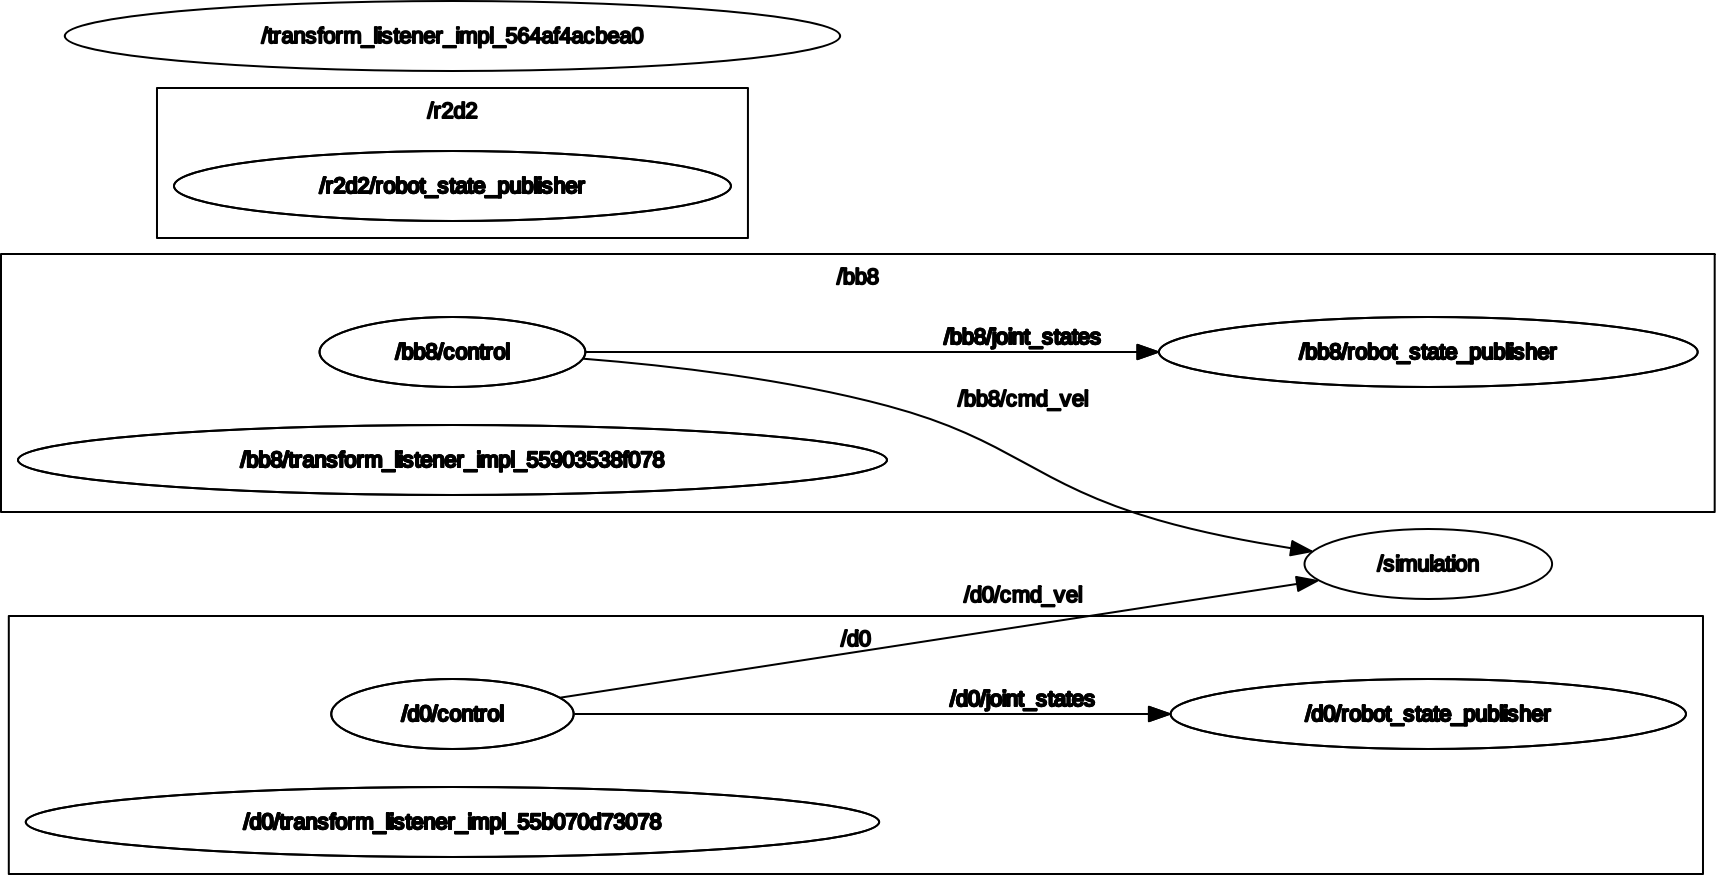
\includegraphics[width=.8\linewidth]{rosgraph}
\end{center}

\newpage

\section{Writing the node}

The node is already more or less setup as \okttt{control_node.cpp}. For now it does exactly nothing. BB8 and D0 should get moving, but also have joints that depend on their current velocity.

The sampling time can be set to $dt = 0.05$ s.

\subsection{Motion control}

You have to use the (already setup) TF listener to get the position of the target with regards to the robot frame. The code from Lab 3 (puppet arm) can be of good use.\\

If the transform is available, we denote $(x,y)$ the linear position error. The control law is then:
\begin{equation*}
   \left\{\begin{array}{ll}
          v &= k_v(x-1) \\
          \omega &= k_\omega \text{arctan2}(y, x)
         \end{array}\right.
\end{equation*}
The gains can be set to around 2 for a good behavior.\\

As usual with 2-0 robots, this command velocity has to be written as a \okttt{geometry_msgs/Twist} message, with the fields \okttt{linear.x} for $v$ and \okttt{angular.z} for $\omega$. 


\subsection{Joint control}

Publishing this command should make the frames move in the simulation, but the 3D models need additional information to be displayed.

Indeed, the controlled robots have 3 joints, the position of which depend on the current velocity as follow:

\begin{center}
 \begin{tabular}{|c|c|}\hline
  Joint name & Position \\\hline
  \okttt{wheel} & $+3.7.v.dt$ (incremental) \\\hline
  \okttt{torso} & $v.\pi/12$\\\hline
  \okttt{neck} & $\omega.\pi/8$\\\hline
 \end{tabular}
\end{center}

Such joint position should be published on the \okttt{joint_states} topic of the robot namespace. You can initialize the joint states message in the node constructor, with the names.\\

Then, when the robot moves, update the \okttt{position} field and the \okttt{header.stamp} from the current time (\okttt{now()}).\\

You can start by publishing only 0 values, that should let the 3D models display correctly.

\section{The launch file}

The launch file should run the node twice, so that BB8 follows R2D2 and D0 follows BB8. Each node should be run in the corresponding robot namespace. The robot name and target should be passed as node parameters, that will be used to know which frames to use in the control.
\newpage
\section{Tips}

Compile the code once using \okttt{colbuild --packages-select ros2_2020}. Then, use \okttt{gqt} in the package folder to configure QtCreator. Do not forget to use it with ROS 2 setup.\\

In order to efficiently debug your code, it is strongly advised to write the node in a specific way to have BB8 follow R2D2. This node should do all necessary things with hard-coded parameters and topics.\\
You can then make it generic and run it through the launch file.\\

Feel free to have a look at the \okttt{basic_node.cpp} from the lab templates.\\

Declaring node parameters is detailed in online tutorials and in my slides.\\

You can use the \okttt{simple_launch} package to write the launch files.\\

% 
% \subsection{Le simulateur}
% 
% Lancez \okttt{midwa.launch}:
% \begin{center}\defaultstyle
% \begin{lstlisting}
% roslaunch ecn_ros2015 midwa.launch
% \end{lstlisting}
% \end{center}
% 
% \def\vx{v_x}
% \def\wz{\omega_z}
% 
% RViz est lancé avec trois robots mobiles plans.
% \begin{itemize}
%  \item Un robot type BB-8 qui suit une trajectoire prédéfinie
%  \item Deux robots type R2-D2 qui sont pour l'instant immobiles
% \end{itemize}Ces robots évoluent en $(x,y,\theta)$ et sont commandés avec une vitesse linéaire $\vx$ et angulaire $\wz$.
% 
% \subsection{Nodes et topics}
% 
% Le node \okttt{simulator} rend compte du déplacement des trois robots. Celui de BB-8 est imposé, les autres dépendent d'une consigne de vitesse.\\
% Chaque robot publie sa position sur le topic \okttt{robot\#/pose} (\okttt{\#} étant un nombre entre 1 et 3) et souscrit à une consigne de vitesse sur le topic \okttt{robot\#/cmd}.\\
% Pour plus d'information, les nodes et topics sont visualisables avec \okttt{rqt_graph} et accessibles via les commandes \okttt{rosnode} et \okttt{rostopic}.
% 
% Les topics qui nous intéressent sont :
% \begin{enumerate}
%  \item Les topics de position (\okttt{robot\#/pose}), sur lesquels sont publiés des messages de type \okttt{geometry_msgs/Pose2D} dont la structure est :
%  \begin{center}\defaultstyle
% \begin{lstlisting}
% float64 x
% float64 y
% float64 theta
% \end{lstlisting}
% \end{center}
% \item Les topics de consigne (\okttt{robot\#/cmd}), sur lesquels le simulateur attend des messages de type \okttt{geometry_msgs/Twist} de structure : 
%  \begin{center}\defaultstyle
% \begin{lstlisting}
% geometry_msgs/Vector3 linear
%   float64 x
%   float64 y
%   float64 z
% geometry_msgs/Vector3 angular
%   float64 x
%   float64 y
%   float64 z
% \end{lstlisting}
% \end{center}
% \end{enumerate}
% 
% Le simulateur ne prend en compte que les champs \okttt{linear.x} (vitesse linéaire dans le repère du robot) et \okttt{angular.z} (vitesse angulaire).
% 
% \section{Objectifs}
% 
% Le travail demandé est d'écrire :
% \begin{itemize}
%  \item Un node qui permet à un robot d'en suivre un autre à une distance donnée
%  \item Un launchfile pour exécuter deux fois le node ci-dessus, afin que les trois robots se suivent
% \end{itemize}
% 
% \subsection{Écriture du node}
% 
% Le node principal est à écrire en C++\footnote{on modifiera le fichier \okttt{CMakeLists.txt} afin de le compiler}.
% Créer le fichier directement dans le dossier \okttt{ecn_midwa}.\\
% Ce node doit :
% \begin{enumerate}
%  \item Souscrire à deux topics de pose (type \okttt{geometry_msgs/Pose2D})
%  \begin{enumerate}
%   \item Le premier est nommé \okttt{current} et correspond à la pose du robot piloté
%   \item Le deuxième est nommé \okttt{target} et correspond à la pose du robot visé
%  \end{enumerate}
%  \item Publier sur un topic de commande en vitesse (type \okttt{geometry_msgs/Twist}), nommé \okttt{cmd}
% \end{enumerate}
% \newpage
% Les deux poses courante $(x_c,y_c,\theta_c)$ et désirée $(x_t,y_t,\theta_t)$ sont représentées en \Fig{schema}.
% \begin{figure}[h]\centering
%  \includegraphics[width=.5\linewidth]{schema}
%  \caption{Poses courante et désirée. Vitesses linéaire $\vx$ et angulaire $\omega_z$.}
%  \label{schema}
% \end{figure}
% 
% La loi de commande $(\vx,\wz)$ permettant au robot contrôlé de s'approcher à une distance $d$ du robot cible est calculée avec l'algorithme suivant :
% \begin{enumerate}
%  \item Calcul de l'erreur cartésienne entre la cible et le robot courant :
%  \begin{equation*}
%   \left\{\begin{array}{ll}
%           dx &= x_t - x_c \\
%           dy &= y_t - y_c
%          \end{array}\right.
%  \end{equation*}
%  \item Calcul de l'erreur angulaire (à remettre dans $[-\pi,\pi]$ si besoin) :
%   \begin{equation*}
%   \alpha = \arctan2(dy, dx) - \theta_c
%  \end{equation*}
%  \item Calcul de l'erreur suivant $x$ dans le repère courant :
%    \begin{equation*}
%   \rho= dx\cos\theta_c + dy\sin\theta_c - d
%  \end{equation*}où $d$ est la distance à laquelle on veut se placer par rapport à la cible.
%  \item Loi de commande proportionnelle :
%   \begin{equation*}
%   \left\{\begin{array}{ll}
%           \vx &= k_\rho\rho \\
%           \wz &= k_\alpha \alpha
%          \end{array}\right.
%  \end{equation*}où $k_\rho$ et $k_\alpha$ sont des gains.
% \end{enumerate}
% On utilisera les valeurs suivantes pour cette application :
%  \begin{equation*}
%   \left\{\begin{array}{ll}
%           d &= 1 \\
%           k_\rho &= 2.7 \\
%           k_\alpha &= 2.9
%          \end{array}\right.
%  \end{equation*}
% La consigne $(\vx,\wz)$ est à écrire ensuite dans un message de type \okttt{geometry_msgs/Twist} et à publier sur le topic \okttt{cmd}.
% \newpage
% 
% \subsection{Écriture du launchfile}
% 
% Le node ci-dessus utilise des topics génériques, il convient donc de le lancer via un launchfile en utilisant la fonction \okttt{remap} pour l'application qui nous intéresse.\\
% 
% Écrire un launchfile permettant au robot 2 de suivre le robot 1, et au robot 3 de suivre le robot 2.\\
% 
% Pour simplifier le développement du node on pourra dans un premier temps écrire en dur les topics permettant au robot 2 de suivre le robot 1.
% 
% 
% 



\end{document}
